% !TeX root = RJwrapper.tex
\title{Working with figure environments in texor}
\author{by Abhishek Ulayil}

\maketitle

\abstract{
This is a small sample article to demonstrate usage of \CRANpkg{texor} to convert figure environments.
}

\section{Introduction}

Images are an essential component of any article, however, due to the differences in support for various graphic formats between LaTeX and markdown/HTML we need to fall back on raster graphics. 
The support for different image formats across markup languages is summarized in Table~\ref{table:1}.

\begin{table}[htbp]
\centering
\begin{tabular}{l | llll }
 \hline
 Graphics Format & LaTeX & Markdown & Rmarkdown & HTML \\
 \hline
 PNG       & Yes & Yes & Yes & Yes \\
 JPG       & Yes & Yes & Yes & Yes \\
 PDF       & Yes & No & No & No \\
 SVG       & No & Yes & Yes & Yes \\
 Tikz      & Yes & No & Yes & No \\
 Algorithm & Yes & No & No & No \\
\hline
\end{tabular}
\caption{Image Format support in various Markup/Typesetting Languages}
\label{table:1}
\end{table}


\section{Image with width parameters}

The following code includes an image with width parameters, producing the output in Figure~\ref{figure:rlogo}.

\begin{verbatim}
\begin{figure}[htbp]
  \centering
  
\includegraphics[width=0.35\textwidth]{Rlogo-5.png}
  \caption{The logo of R.}
  \label{figure:rlogo}
\end{figure}
\end{verbatim}

\begin{figure}[htbp]
  \centering
  
\includegraphics[width=0.35\textwidth]{Rlogo-5.png}
  \caption{The logo of R.}
  \label{figure:rlogo}
\end{figure}

This is the most basic example of figure.

\section{Images in PDF format}

The following code includes an image in PDF format, shown in Figure \ref{fig:normal}.

\begin{verbatim}
\begin{figure}[htbp]
  \centering
  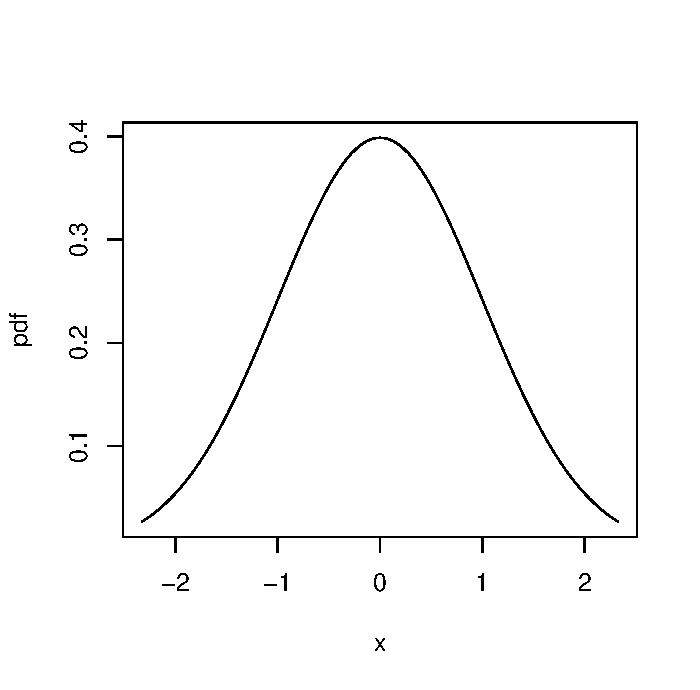
\includegraphics[width=0.5\textwidth]{normal}
  \caption{PDF of a normal distribution}
  \label{fig:normal}
\end{figure}
\end{verbatim}
\begin{figure}[htbp]
  \centering
  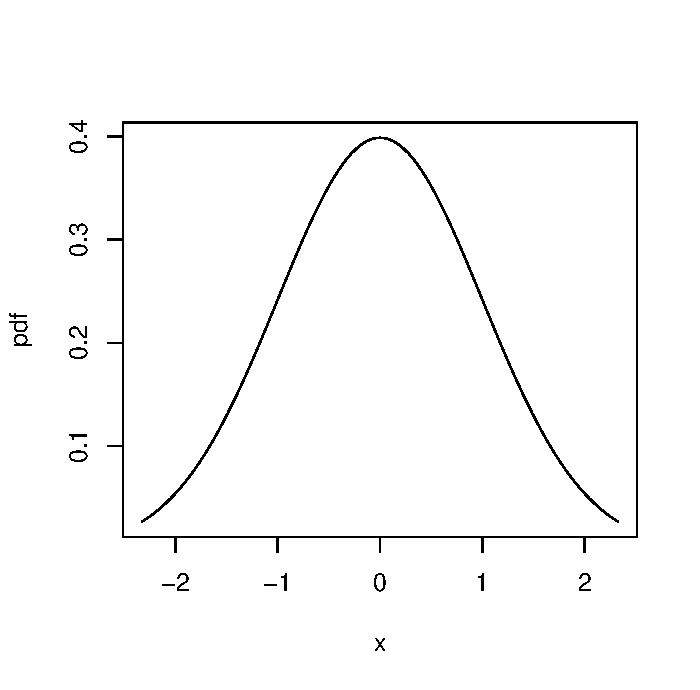
\includegraphics[width=0.5\textwidth]{normal}
  \caption{PDF of a normal distribution}
  \label{fig:normal}
\end{figure}

\section{Multiple images}
 Pandoc v3 and above now support a new \code{Figure} object \citep{pandoc} which supports multiple 
 images side by side or in a grid format. The following subsections demonstrate these capabilities.
%% Two images side by side
\subsubsection{Two or more Images side by side}
\begin{verbatim}
\begin{figure}[htbp]
  \centering
  
\includegraphics[width=0.45\textwidth]{Rlogo-5.png}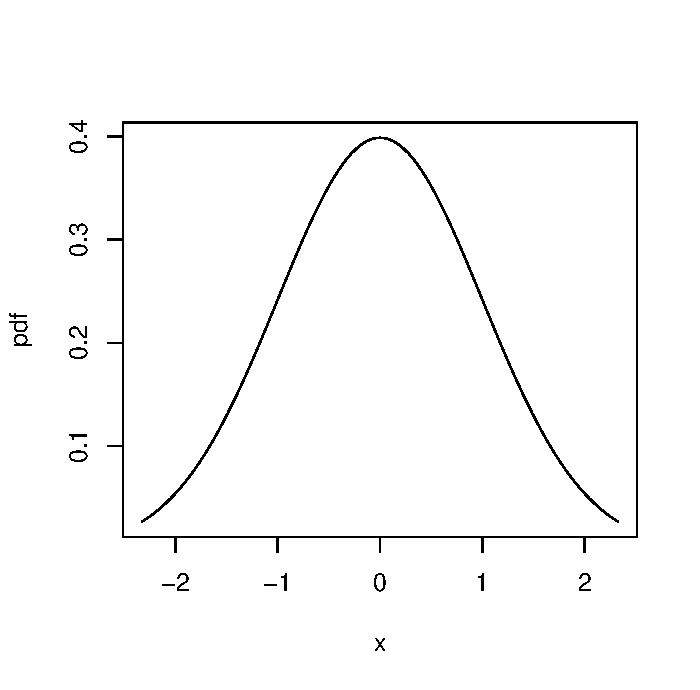
\includegraphics[width=0.45\textwidth]{normal}
  \caption{Images side by side}
  \label{fig:twoimages}
\end{figure}
\end{verbatim}

\begin{figure*}[htbp]
  \centering
  
\includegraphics[width=0.45\textwidth]{Rlogo-5.png}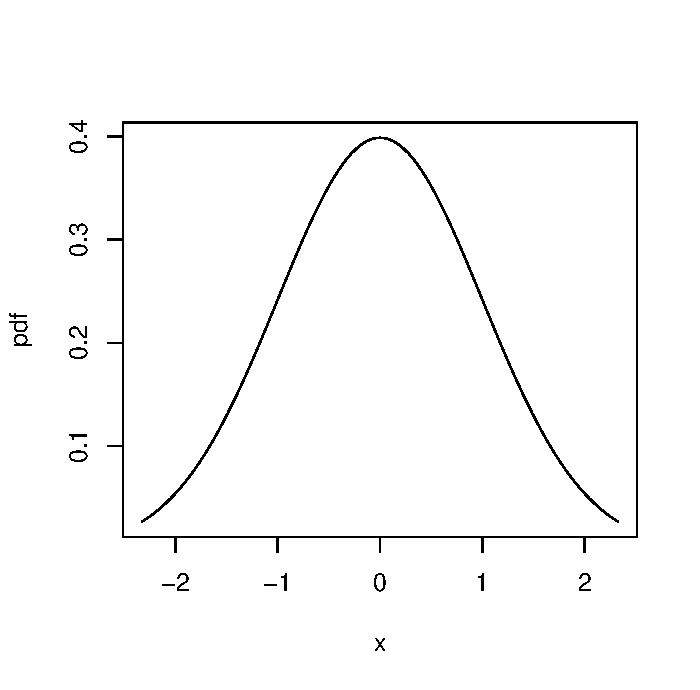
\includegraphics[width=0.45\textwidth]{normal}
  \caption{Images side by side}
  \label{fig:twoimages}
\end{figure*}

%% Four images in a grid
\subsubsection{Four Images in a grid}

\begin{verbatim}
\begin{figure}[htbp]
  \centering
  
\includegraphics[width=0.45\textwidth]{Rlogo-5.png}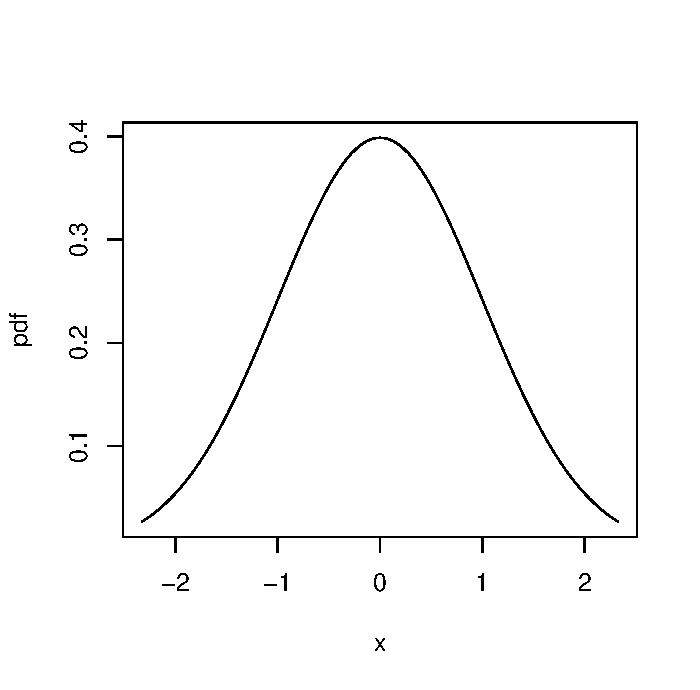
\includegraphics[width=0.45\textwidth]{normal}
  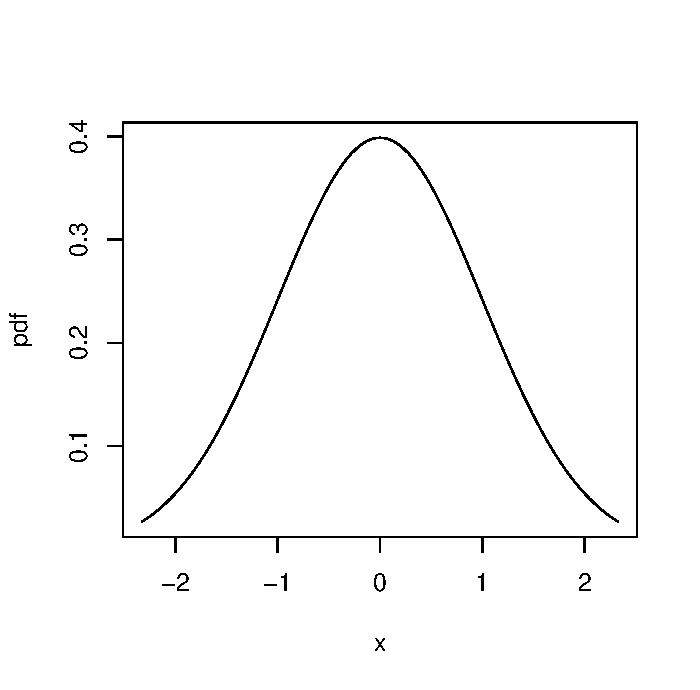
\includegraphics[width=0.45\textwidth]{normal}
\includegraphics[width=0.45\textwidth]{Rlogo-5.png}
  \caption{Multiple images in a grid}
  \label{fig:fourimages}
\end{figure}

\end{verbatim}

\begin{figure}[htbp]
  \centering
  
\includegraphics[width=0.45\textwidth]{Rlogo-5.png}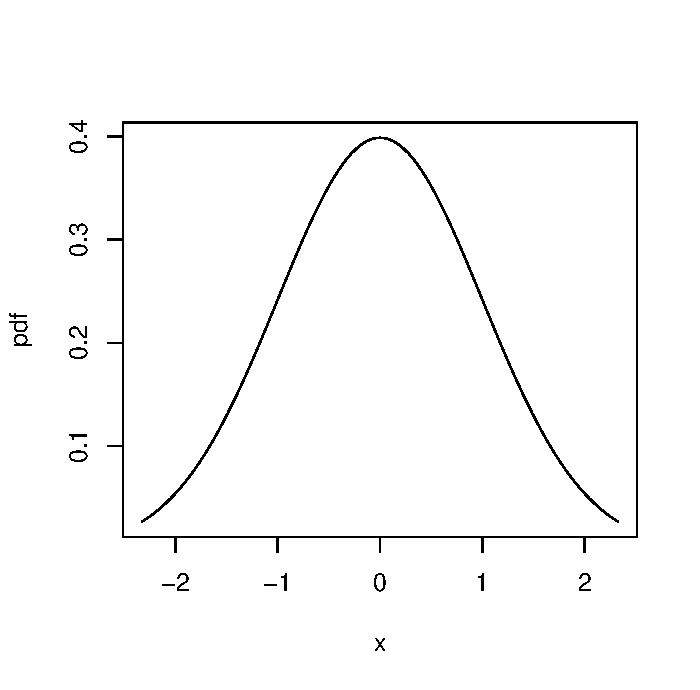
\includegraphics[width=0.45\textwidth]{normal}
  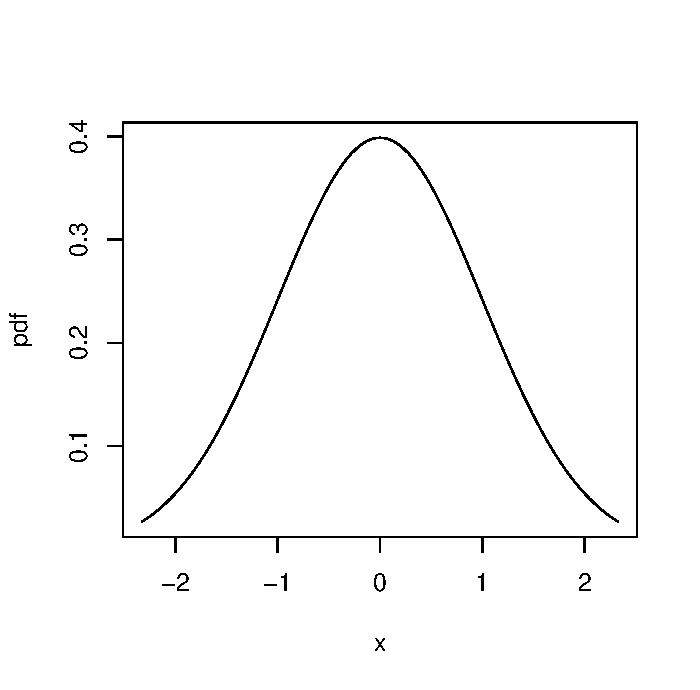
\includegraphics[width=0.45\textwidth]{normal}
\includegraphics[width=0.45\textwidth]{Rlogo-5.png}
  \caption{Multiple images in a grid}
  \label{fig:fourimages}
\end{figure}


\section{Tikz images}

Figure \ref{fig:tikz} shows a tikz image adapted from \citep{casflow}.


An interesting aspect of including a tikz image here is that you can modify the
source and re-convert without making any other changes. Figure will get updated
in the generated html article.

\subsubsection{Tikz Code:}
The image in Figure  \ref{fig:tikz} is a graphical representation of how \pkg{texor} handles tikz images:

\begin{itemize}
\item Figures containing tikz images are isolated.
\item Tikz libraries are fetched from the wrapper file.
\item The Tikz code section is isolated into a standalone LaTeX file and compiled.
\item The compiled LaTeX file generates a PDF Image.
\item This is converted to PNG format for embedding in the HTML output.
\item \verb|\includegraphics{tikz/somefigure.png}| is added to the figure environment.
\item A lua filter removes redundant text the figure environment.
\end{itemize}

If you use \pkg{texor} to convert your articles using \verb|texor::latex_to_web()| with \verb|temp_mode=TRUE|(it is \verb|TRUE| by default). The resultant Rmarkdown/HTML file will not modify the contents of your LaTeX file. In this case you can keep reloading the article after making changes to the tikz images, without having to do the above steps manually in case you are converting the article by hand.

\begin{figure*}

%% Generated Image will included as a PNG above
  \centering
\tikzstyle{process} = [rectangle, rounded corners,
minimum width=3cm, 
minimum height=1cm,
text centered, 
draw=black]
\tikzstyle{arrow} = [thick,->,>=stealth]
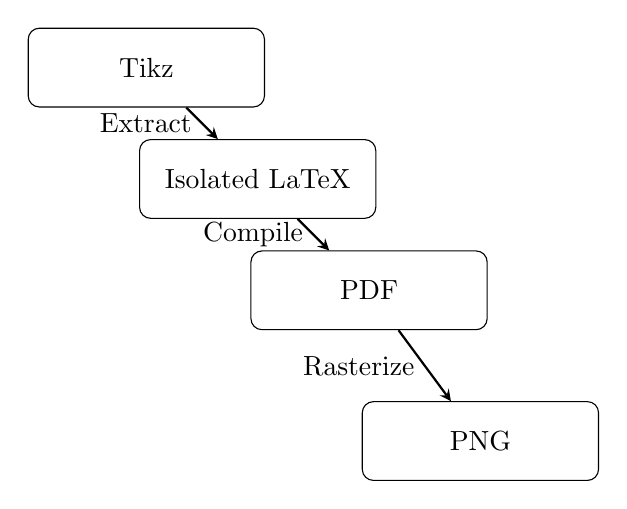
\begin{tikzpicture}[node distance=2cm]
%Nodes
\node (start) [process] {Tikz};
\node (isolate) [process, below right of=start] {Isolated LaTeX};
\node (pro1) [process, below right of=isolate] {PDF};
\node (pro2) [process, below right of=pro1, yshift=-0.5cm] {PNG};
% arrows
\draw [arrow] (start) -- node[anchor=east] {Extract} (isolate);
\draw [arrow] (isolate) -- node[anchor=east] {Compile} (pro1);
\draw [arrow] (pro1) -- node[anchor=east] {Rasterize} (pro2);

\end{tikzpicture}
\caption{Tikz Image example}
  \label{fig:tikz}
\end{figure*}


\section{Algorithm2e diagrams}

Diagrams and images using the \code{algorithm2e} environment are supported, these will be numbered differently.
We strongly suggest to use "alg:" in labels for best results. 
Algorithm \ref{alg:how} is an example from the \CRANpkg{algorithm2e} vignette \cite{algoexample}.


\begin{algorithm}[htbp]
\SetAlgoLined
\KwData{this text}
\KwResult{how to write algorithm with \LaTeX2e }
initialization\;
\While{not at end of this document}{
read current\;
\eIf{understand}{
go to next section\;
current section becomes this one\;
}{
go back to the beginning of current section\;
}
}
\caption{How to write algorithms}
  \label{alg:how}
\end{algorithm}

\section{Other elements in figure objects}

Figures can also house non-image environments like code blocks and wide tables. This is 
one aspect where the converted articles differ between PDF and HTML formats. Code blocks 
in figure environments would have numbering and caption of the form "Figure x:" in the PDF output. However, 
when the code blocks are converted to R Markdown, they are numbered as "CodeBlock x:".
This distinguishes them from normal images and matches with the authors' vision more appropriately. 

As for the inclusion of wide tables, since the figure houses two different tabular environments with the same caption,
this would be treated by pandoc as two different tables sharing the same caption. This would not be the best solution hence, the \pkg{texor} package uses Figure environment to house the widetables.
This way they are distinguished well from normal tables, also the numbering scheme is seperated from figures "WideTable x:".

However one important thing to note is, the reference links and reference numbering would be shared with ones of the figures. So the changes that the package makes are cosmetic to captions. Like CodeBlock 1 below refers to \ref{code:example}. The number should have been 1 but instead it is 7.

\begin{figure}[htbp]
\begin{center}
\begin{verbatim}
code_in_figure <- function() {
  if (pandoc_version >= 3) {
    print("code in figure supported")
  }
  else {
    print("code in figure not supported")
  }
}
\end{verbatim}
\caption{ Example Code inside Figure environment}
\label{code:example}
\end{center}
\end{figure}
\section{Summary}

In summary the \CRANpkg{texor} package supports:
\begin{itemize}
\item Almost all image formats in LaTeX.
\item Algorithm and tikz as well in some capacity.
\item Multiple images in grid,side-by-side configuration.
\item Image Captions with Numbering and Labelling.
\end{itemize}



\begin{thebibliography}{4}
    \providecommand{\natexlab}[1]{#1}
    \providecommand{\url}[1]{\texttt{#1}}
    \expandafter\ifx\csname urlstyle\endcsname\relax
      \providecommand{\doi}[1]{doi: #1}\else
      \providecommand{\doi}{doi: \begingroup \urlstyle{rm}\Url}\fi
\bibitem[Cassidy(2013)]{casflow}
Josh Cassidy
\newblock LaTeX Graphics using TikZ: A Tutorial for Beginners (Part 3)—Creating Flowcharts
\newblock \emph{Overleaf tutorials} \penalty0 2013
\newblock URL \url{https://www.overleaf.com/learn/latex/}

\bibitem[Fiorio (2017)]{algoexample}
Christophe Fiorio
\newblock algorithm2e.sty — package for algorithms, release 5.2
\newblock \emph{CTAN},\penalty0 2017
\newblock URL \url{https://mirror.kku.ac.th/CTAN/macros/latex/contrib/algorithm2e/doc/algorithm2e.pdf}

\bibitem[Krewinkel, Lucero (2023)]{pandoc}
Albert Krewinkel and Aner Lucero
\newblock pandoc 3.0 Release notes
\newblock \emph{pandoc} \penalty0 2023
\newblock URL \url{https://pandoc.org/releases.html}

\end{thebibliography}


\address{%
Abhishek Ulayil\\
Student, Institute of Actuaries of India\\%
Mumbai, India\\
ORCiD: 0009-0000-6935-8690\\
}
